\documentclass{article}

\usepackage{graphicx}
\usepackage{wrapfig}
\usepackage{titling}
\usepackage[RPvoltages]{circuitikz}
\usepackage{tikz}
\usepackage{siunitx}
\usepackage{physics}
\usepackage{amsmath}
\usepackage{pgfmath}
\usepackage{pgfplots}
\usepackage{mathdots}
\usepackage{yhmath}
\usepackage{cancel}
\usepackage{color}
\usepackage{array}
\usepackage{multirow}
\usepackage{amssymb}
\usepackage{gensymb}
\usepackage{tabularx}
\usepackage{booktabs}
\usepackage{capt-of}
\usepackage{pgfkeys}
\usepackage[export]{adjustbox}
\usepackage[labelformat=empty]{caption}
\usepackage{hyperref}
\usepackage{verbatim}
\usetikzlibrary{patterns}
\usetikzlibrary{shadows.blur}
\usetikzlibrary{positioning, shapes, fadings, calc}
\usepgfplotslibrary{fillbetween}

\setlength{\droptitle}{-10em}
\title{Nonvolatile Storage with Magnetic Core Memory}
\author{Jack Brower}
\date{April 2021}

\renewcommand{\arraystretch}{1.2} 
\pgfplotsset{width=7cm,height=9cm,plotstyle/.style={line width=1.2pt,smooth,samples=100,domain=-0.05:1.01}} 

\begin{document}

\maketitle

\section{Introduction}
In the 1940s, the US Navy commissioned MIT to create a flight simulator to train incoming bomber pilots. Titled \emph{Project Whirlwind}, this flight simulator would be the first computer to use modern data storage techniques by utilizing the properties of magnetic polarity to store data in the form of bits, 1s and 0s. The researchers of \emph{Project Whirlwind} used relatively simple electric and magnetic mechanics to manipulate the state of ferrite cores in order to quickly store data as a form of early random-access memory, not unlike modern RAM.\textsuperscript{8}

\begin{wrapfigure}{r}{0.4\textwidth}
  \includegraphics[width=\linewidth]{img/bookcoregrid.png}
  \caption{\small \emph{fig 1. Ferrite core grid.\textsuperscript{3}}}
\end{wrapfigure}

\noindent The basic setup for a computer-model core memory bank is with two parallel rows of current-carrying wire, where any point which the wires cross creates a ferrite core node. This allows for any individual core to be manipulated by sending an on/off signal to two corresponding wires, e.g. $(X_2, Y_3)$. This changes the state of the core on said node. The ferrite cores then undergo magnetic hysteresis depending on the strength of their field relative to the magnetic flux. As seen in \emph{figure 2}, there is a point on either side where magnetic flux $B$ grows exponentially, and then ``levels off". The point at which magnetic flux ``levels off" is the point where the state of the magnet changes to a 1 or a 0. On any given hysteresis graph, this point is found at the intersection where $B=0$. This method of storage is also used in modern hard disk drives, where individual bits

\begin{wrapfigure}{l}{0.4\textwidth}
  \includegraphics[width=\linewidth]{img/hysteresis-graph.png} 
  \caption{\small \emph{fig 2. Hysteresis graph.\textsuperscript{3}}}
\end{wrapfigure}

\noindent are stored on a film of ferromagnetic material, and pixels on the film are aligned to a magnetic pole through the process of hysteresis.\textsuperscript{3} In the case of core memory, the process of reading the cores destroys the data stored on the cores. However in this project, the cores are written to so long as there is power to the circuit, even without constant user input. This means that the circuit created is both non-volatile, meaning it maintains its state with or without power, and non-destructive, meaning reading the data does not interfere with hysteresis.

\clearpage\newpage\section{Methods}
Magnetic core memory operates on the principle of the Amp\'ere-Maxwell law (a revision of Amp\'ere's Circuital Law), which states that a current carrying wire produces an encircling magnetic field. The related equation is:

\[ \nabla \cross \vb{B} = \mu_0\vb{J} + \mu_0\varepsilon_0 \frac{\partial\vb{E}}{\partial t} \]

\noindent Where Maxwell's addition of the term $\mu_0\varepsilon_0 \frac{\partial\vb{E}}{\partial t}$ accounts for electric displacement\textsuperscript{2}, which is necessary to explain the function of the process of hysteresis in the ferromagnetic loop, see \emph{fig. 2}. Individual bits a core memory module are stored in square-loop ferrite cores, which are looped in a certain number of wire, depending on the configuration. As per the Amp\'ere-Maxwell law\textsuperscript{3}, the magnetic cores undergo hysteresis, which is the alignment of atomic dipoles towards a certain polarity. In computer configurations, the state of the magnet is read by a sense wire (see \emph{fig. 1}), which interferes with the state of the magnet and destroys the data held by the ferrite core. In the configuration used in this project, the charge of the cores themselves are used to store the state of a pair of LEDs in a JK latch circuit in a non-destructive and non-volatile way.

\begin{figure}[h]\centering
\begin{comment}
\begin{circuitikz}[decoration={coil}]
  % Left side
  \draw (-3,-3) 
  to node[ground]{} (-3,-3);
  \draw (-3,-3)
  to node[nosshape, xscale=-1]{} (-4,-3)
  to [short,-o] (-4,-3) node[below] {$\mathrm{K}$}
  to (-4,-3) -- (-4,-1)
  to (-3.5,-1) node[npn, anchor=west]{2N3638A} 
  ;
  \draw (-2.660,-1.775) node[ground]{};
  \draw (-4.5,-2.5)
  to (-4,-2.5) -- (-4.5,-2.5)
  to [R=$10 \text{ k}\ohm$] (-4.5,-1)
  to node[rground, label=\raisebox{2.5ex}{$\mathrm{V_{cc}}$}, yscale=-1]{} (-4.5,-1)
  ;
  \draw (-4,-1)
  to [R=$1 \text{ k}\ohm$] (-4,3)
  ;
  \draw (-4,3)
  to [short,-o] (-4,3) node[above] {$\mathrm{\bar Q}$}
  to (-4,3) -- (-4.5,3)
  to (-4.5,3) -- (-4.5,3.5)
  to [R=$10 \text{ k}\ohm$] (-4.5,4.7)
  to (-4.5,4.7) -- (-4.5,5)
  to (-4.5,5) -- (-4.25,5)
  to [leD] ++(1.5,0);
  \draw (-2.75,5) node[ground]{} (-2.75,4);
  \draw (-3.95,3)
  to (-3.95,3) -- (-2,3)
  to [R=$100 \ohm$] (-2,5)
  to node[rground, label=\raisebox{2.5ex}{$\mathrm{V_{cc}}$}, yscale=-1]{} (2,5);

  % Right side. For labels to be on the right they must be drawn up -> down. See first resistor for example.
  \draw (3,-3) 
  to node[ground]{} (3,-3)
  to node[nosshape, xscale=1]{} (4,-3)
  to [short,-o] (4,-3) node[below] {$\mathrm{J}$}
  to (4,-3) -- (4,-1)
  to (3.5,-1) node[npn, anchor=west, xscale=-1, label={[xshift=-5ex, yshift=-1.4ex]2N3638A}]{}
  ; 
  \draw (2.660,-1.775) node[ground]{};
  \draw (4.5,-1)
  to node[rground, label=\raisebox{2.5ex}{$\mathrm{V_{cc}}$}, yscale=-1]{} (4.5,-1)
  to [R=$10 \text{ k}\ohm$] (4.5,-2.5) -- (4,-2.5)
  ;
  \draw (4,3)
  to [R=$1 \text{ k}\ohm$] (4,-1)
  ;
  \draw (4,3)
  to [short,-o] (4,3) node[above] {$\mathrm{Q}$}
  to (4,3) -- (4.5,3)
  to (4.5,3) -- (4.5,3.5);
  \draw (4.5,4.7)
  to [R, label=$10 \text{ k}\ohm$] (4.5,3.5);
  \draw (4.5,4.7)
  to (4.5,4.7) -- (4.5,5)
  to (4.5,5) -- (4.25,5)
  to [leD, mirror] ++(-1.5,0);
  \draw (2.75,5) node[ground]{} (2.75,4);
  \draw (3.95,3)
  to (3.95,3) -- (2,3);
  \draw (2,5) to [R=$100 \ohm$] (2,3);

  % Ferrite cores
  \draw (-1.5,1.25) circle[radius=.2cm] circle[radius=.4cm];
  \draw (1.5,1.25) circle[radius=.2cm] circle[radius=.4cm];
  \begin{scope}[scale=0.5]
    \draw[decorate, decoration={aspect=.5, segment length=2mm, amplitude=2mm}] (3.5,1.6) coordinate (c) --node[midway,left=0.5cm]{} + (0,2) coordinate (d);
    \draw[decorate, decoration={aspect=.5, segment length=2mm, amplitude=2mm}] (-3.5,1.6) coordinate (c) --node[midway,left=0.5cm]{} + (0,2) coordinate (d);
  \end{scope}
  \draw (-1.755,.8) node[ground]{};
  \draw (1.755,.8) node[ground]{};

\end{circuitikz}
\end{comment}
\includegraphics[width=9cm]{img/flipflop.png}
\caption{\small\emph{fig 3. Modified JK latch circuit. The center loops are 4mm square-loop ferrite cores.\textsuperscript{9}}}
\end{figure}

\newpage

\noindent A JK latch is a type of circuit that operates on the principle of logic gates, which are themselves circuits that change states based on their inputs. The above circuit can be represented with logic gates as:
\newline\newline
\noindent
  \begin{minipage}[b]{0.5\linewidth}
  \centering
  \begin{circuitikz}[scale=0.5, transform shape]
    
    % AND logic gates
    \node[ieeestd and port] (and1) at (0,2) {AND};
    \node[ieeestd and port] (and2) at (0,-2) {AND};
    % NOR logic gates
    \draw (and1.out) -- ++(2.5,0) node[ieeestd nor port,anchor=in 1] (nor1) {NOR};
    \draw (and2.out) -- ++(2.5,0) node[ieeestd nor port,anchor=in 2] (nor2) {NOR};
    \draw (nor1.in 2) -| ++ (-0.2,-0.85) -- ++(3,-1.5) coordinate(a) |- (nor2.out);
    \draw (nor2.in 1) -| ++ (-0.2,0.85) -- ++(3,1.5) |- (nor1.out);
    % Labels
    \draw (and1.in 2) -- ++(-0.75,0) node[left]{J};
    \draw (and2.in 1) -- ++(-0.75,0) node[left]{K};
    \draw (nor1.out -| a) -- ++(0.75,0) node[right]{$\mathrm{\bar Q}$};
    \draw (nor2.out -| a) -- ++(0.75,0) node[right]{$\mathrm{Q}$};
    % Additional
    \draw (and1.in 1) -- ++(0,.5)
        to (6.7,2.8) to (6.7,1.715)
    ;
    \draw (and2.in 2) -- ++(0,-.5)
        to (6.7,-2.8) to (6.7,-1.715)
    ;
  \end{circuitikz}
\end{minipage}\hfill
\begin{minipage}[b]{0.5\linewidth}
    \centering
    {\bfseries\strut Table 1: JK latch truth table}
    \begin{tabular}[b]{|l|l|l|l|}
      \hline
      {\boldmath $\mathrm{J}$} & {\boldmath $\mathrm{K}$} & {\boldmath $\mathrm{Q_{state}}$} & \textbf{Change} \\ \hline
      0            & 0            & $Q$                  & No change       \\ \hline
      0            & 1            & 0                    & Reset           \\ \hline
      1            & 0            & 1                    & Set             \\ \hline
      1            & 1            & $\bar Q$             & Toggle          \\ \hline
    \end{tabular}
\end{minipage}

\begin{center} 
  \small\emph{fig 4. Perfect logic gate diagram and corresponding truth table.} 
\end{center}

\noindent Where the circuit forms four logic gates of two different types, AND and NOR, which have different functions in of themselves depending on their two inputs. For example, a NOR gate would out an electric pulse (1) only if there is no electric signal. An AND gate would send out an electric pulse (1) only if both its inputs have an electric signal. For the circuit above, the state of the JK latch is stored in the two ferrite cores and switch when a different signal is manually sent. This differs from a JK flip-flop in that electric inputs are supplied on a certain frequency by a clock instead of on demand by the user.\textsuperscript{7}
\newline This project will be collecting data based on the output of the circuit itself (that is the state of the LEDs based on the user input of switches J and K) and on the relative change in flux (gauss) of the ferrite cores in both states as it is powered on. As the magnets undergo hysteresis in either state, there should me a measurable difference from the opposite state that is approximately the opposite of its alternate state. Magnetic flux will be measured using a gauss meter with a range of 0.1 mG to 10 mG.
\subsection*{Error Analysis}
The readings given by the gauss meter will be compared three sources: the original paper on magnetic core memory\textsuperscript{1}, the book ``Square-Loop Ferrite Circuitry: Storage and Logic Techniques", and its sister book ``Magnetic Core Storage". These three materials report a reading of the square-loop ferrite cores, when in a 1 or a 0 state, to be $(1800\pm400) \times 10^{-4}$ gauss, which is within the range of the gauss meter. Therefore, the following error analysis can be conducted.

\[\% \; \mathrm{Error} \; = \; \absolutevalue{\frac{G_{theoretical} - G_{experimental}}{G_{theoretical}}} \times 100\]
\[\% \; \mathrm{Error} \; = \; \absolutevalue{\frac{(1800\pm400) \times 10^{-4} \; \mathrm{G} - G_{experimental}}{(1800\pm400) \times 10^{-4} \; \mathrm{G}}} \times 100\]

\noindent Given the uncertainty for $G_{theoretical}$, $G_{theoretical}$ will be calculated such that the measured value is within 0.1 mG of the theoretical, readings permitting.

\newpage\section{Results \& Analysis}
\noindent The created circuit, when powered on, works as follows:
\begin{figure}[h]\centering
\begin{circuitikz}[scale=.75, transform shape]
    
  % AND logic gates
  \node[ieeestd and port] (and1) at (0,2) {AND};
  \node[ieeestd and port] (and2) at (0,-2) {AND};
  % NOR logic gates
  \draw (and1.out) -- ++(2.5,0) node[ieeestd nor port,anchor=in 1] (nor1) {NOR};
  \draw (and2.out) -- ++(2.5,0) node[ieeestd nor port,anchor=in 2] (nor2) {NOR};
  \draw (nor1.in 2) -| ++ (-0.2,-0.85) -- ++(3,-1.5) coordinate(a) |- (nor2.out);
  \draw (nor2.in 1) -| ++ (-0.2,0.85) -- ++(3,1.5) |- (nor1.out);
  % Labels
  \draw (and1.in 2) -- ++(-0.75,0) node[left]{J};
  \draw (and2.in 1) -- ++(-0.75,0) node[left]{K};
  \draw (nor1.out -| a) -- ++(0.75,0) node[right]{$\mathrm{\bar Q}$};
  \draw (nor2.out -| a) -- ++(0.75,0) node[right]{$\mathrm{Q}$};
  % Additional
  \draw (and1.in 1) -- ++(0,.5)
      to (6.7,2.8) to (6.7,1.715)
  ;
  \draw (and2.in 2) -- ++(0,-.5)
      to (6.7,-2.8) to (6.7,-1.715)
  ;
\end{circuitikz}
\caption{\small\emph{fig 5. Real circuit logic gate diagram.}}
\end{figure}

\noindent Which is a perfect match to the theoretical model listed above. Furthermore, the state of the circuit is preserved on a power cycle, which is also in line with the non-volatile properties of a square-loop ferrite core. In other words, the circuit functions exactly as expected.

\noindent The below readings were taken from a distance of no more than five centimeters. Additionally, the readings were recorded in a dim room isolated from electronics excluding the circuit's power supply. Due to the limitations of the gauss meter, readings are only accurate to 0.5 mG. 

\vspace{.3cm}

\noindent
  \begin{minipage}[b]{0.5\linewidth}
  \centering
  \hspace*{-0.1cm}\vspace*{-2cm}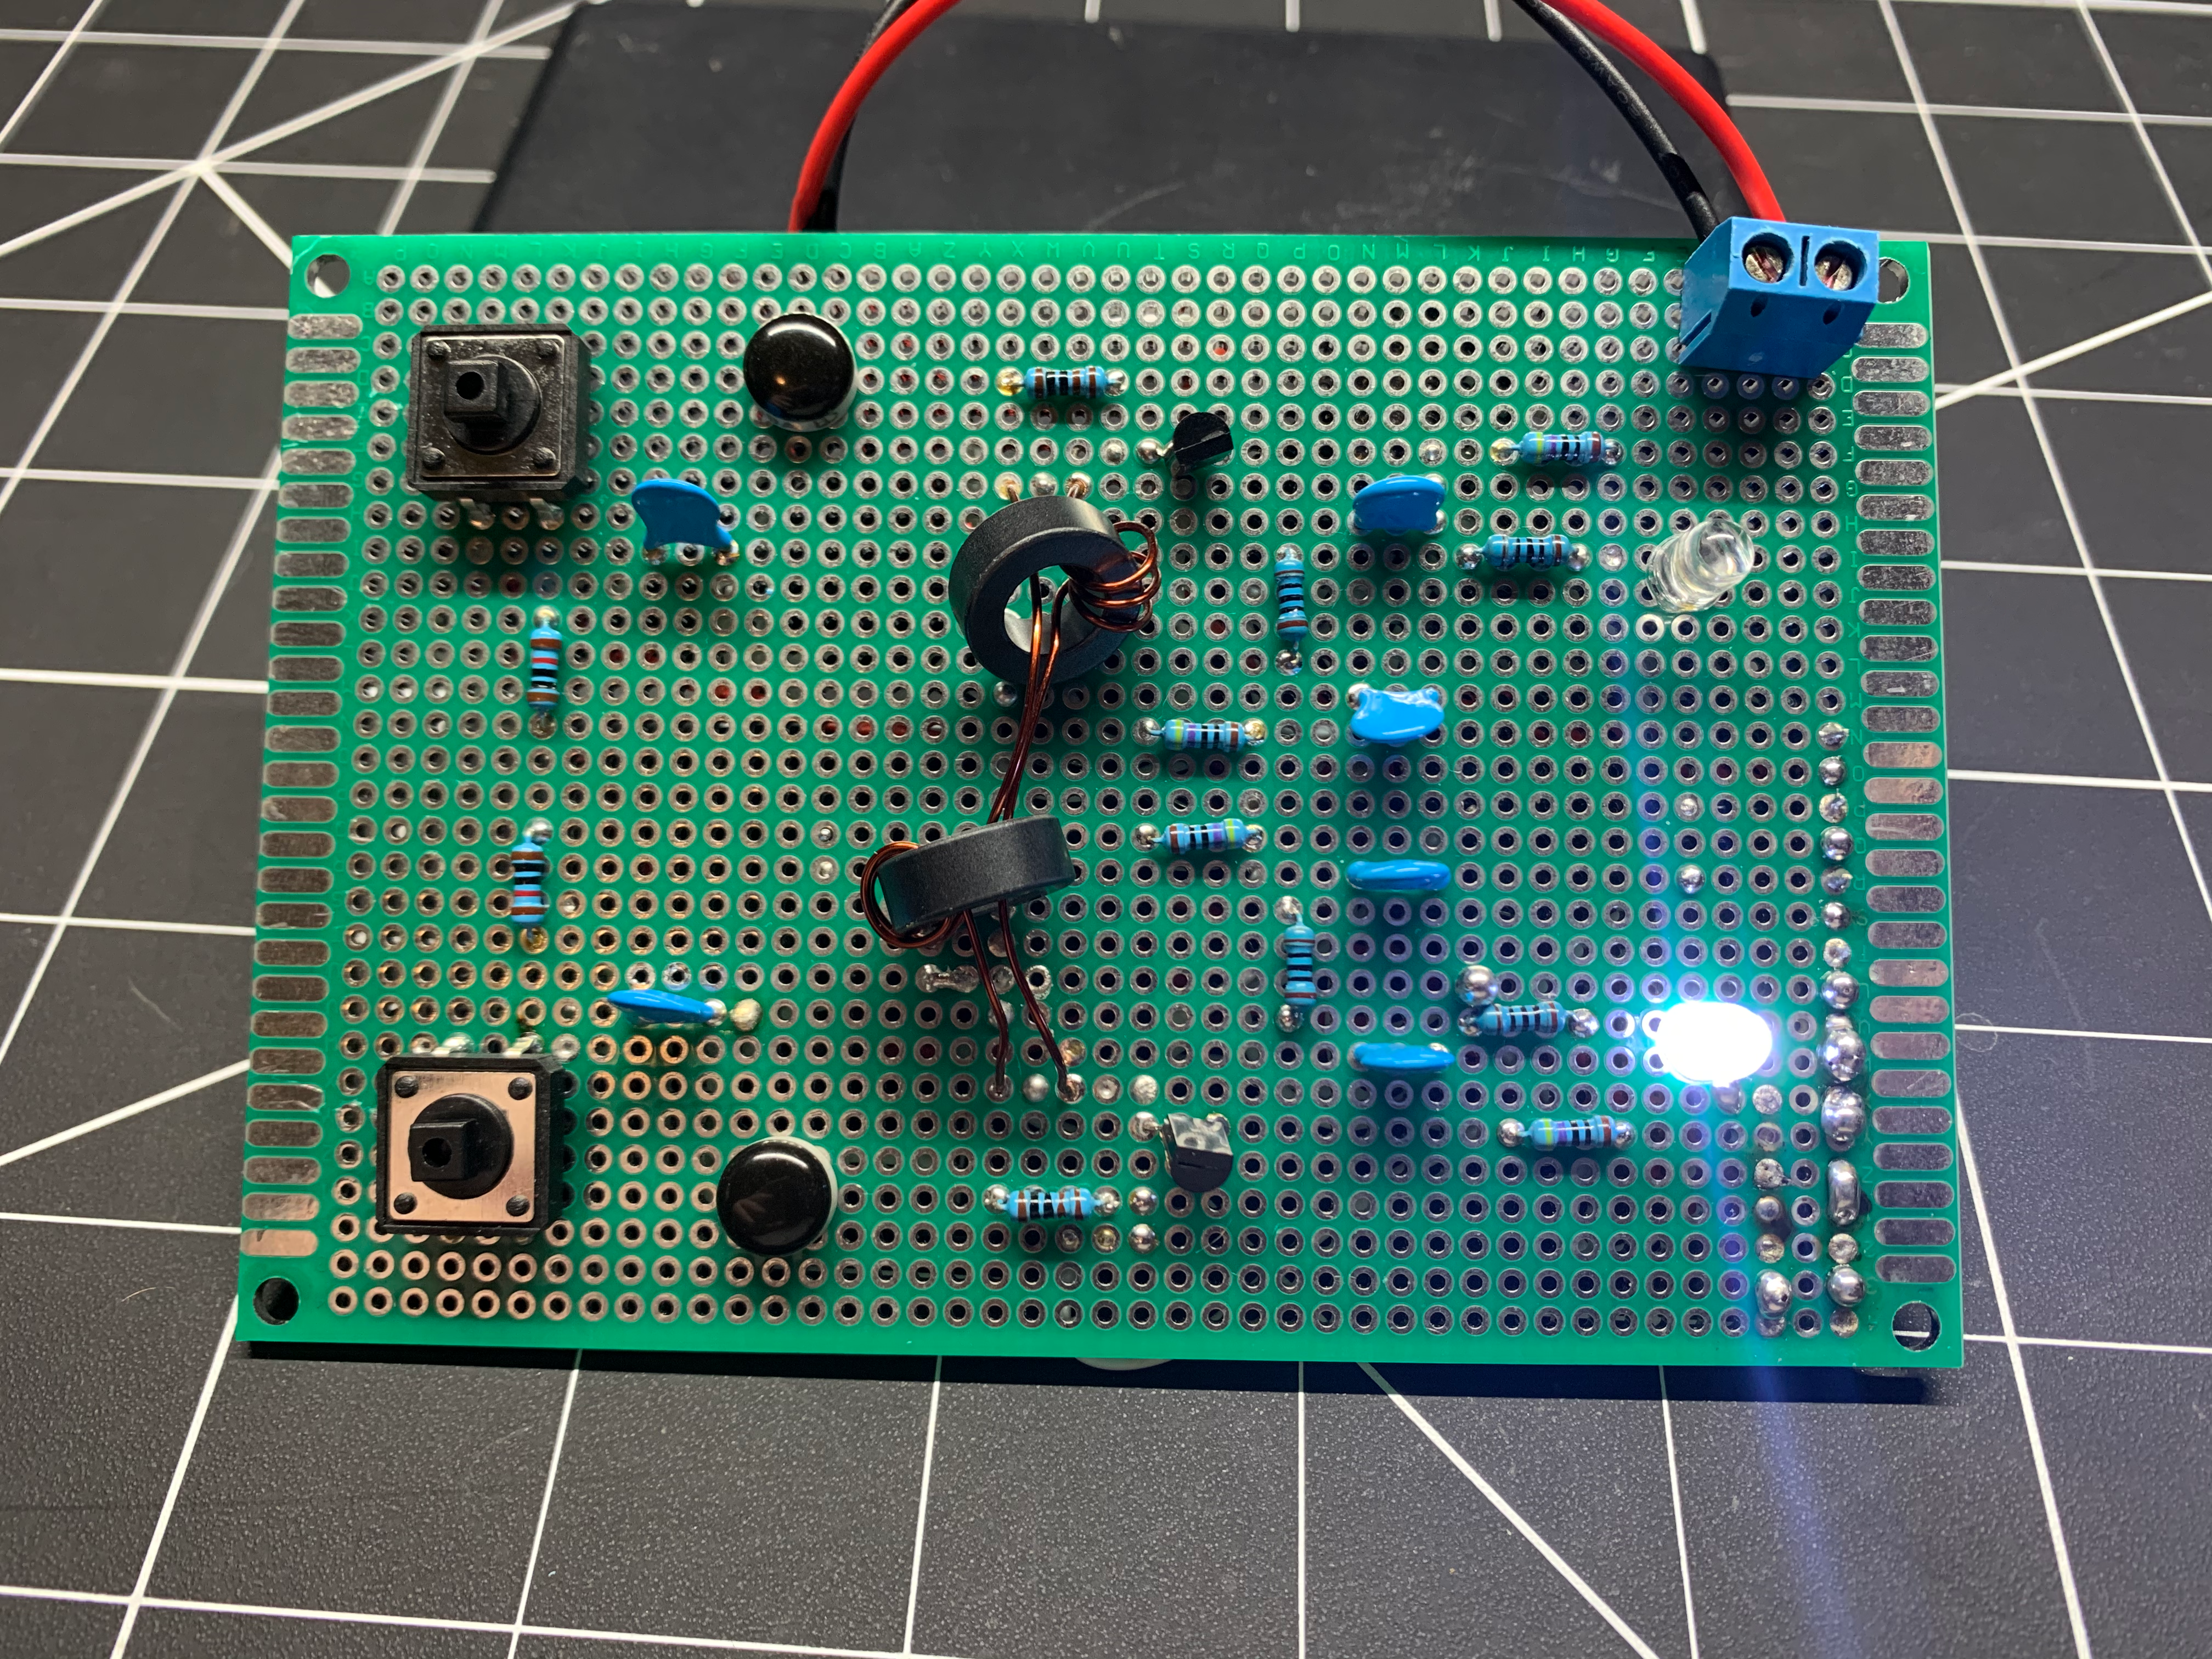
\includegraphics[height=4.5cm]{img/circuitfinished.png}
\end{minipage}\hfill
\begin{minipage}[b]{0.5\linewidth}
      \centering
      {\bfseries\strut Table 2: Gauss readings}
      \begin{tabular}{|l|l|}
      \hline
      \textbf{Left core state}  & \textbf{Flux in gauss} \\ \hline
      0                         & 8 mG                 \\ \hline
      1                         & 8 mG                 \\ \hline \hline
      \textbf{Right core state} & \textbf{Flux in gauss} \\ \hline
      0                         & 8 mG                 \\ \hline
      1                         & 8.5 mG                 \\ \hline
    \end{tabular}
\end{minipage}

\vspace{.3cm}

\begin{center} 
  \small\emph{fig 6. Image of the powered-on circuit with gauss readings.} 
\end{center}

\noindent When compared to the target rating of $1.8 \pm 0.4$ mG, there is a clear discrepancy. Conducting an error analysis reveals the following:

\[\% \; \mathrm{Error_{Left_{0\wedge1}, \; Right_0}} \; = \; \absolutevalue{\frac{2.2 \; \mathrm{mG} - 8 \; \mathrm{mG}}{2.2 \; \mathrm{mG}}} \times 100 = 264\%\] 
\[\% \; \mathrm{Error_{Right_1}} \; = \; \absolutevalue{\frac{2.2 \; \mathrm{mG} - 8.5 \; \mathrm{mG}}{2.2 \; \mathrm{mG}}} \times 100 = 286\%\] 

\newpage\section{Conclusion}
\noindent Unfortunately, the calculated error casts too much doubt on the data for it to be considered accurate. The reason for the difference between this project's data and the data reported in the reports mentioned above is likely due to a number of errors.
\begin{itemize}
  \item The gauss meter is too inaccurate to measure the flux from the magnetic cores.
  \item The data used in sources 1, 3, and 4 is accurate only for a certain size of magnetic cores, or in the computer configuration see in \emph{fig. 1}.
  \item There was background interference from other electronics, outside lights, or other unidentifiable sources. 
  \item The circuit itself or its power supply caused interference, which would be inseparable from the magnetic cores without more precise tools.
\end{itemize}
\noindent Also worth noting is that there was no change in polarity as there should have been according to the above section. The gauss meter used to measure the change in magnetic flux does not represent polarity, only magnitude, and therefore the polarity was not considered in recording or in the error analysis.
\newline
\noindent Considering the circuit functioned as intended, and similar readings were given for both states for either magnetic core, the most plausible explanation is that there is a fundamental flaw in the way the readings were recorded and compared. That said, the lab succeeded in demonstrating basic concepts of circuits, magnets, and data storage.

\begin{figure}[h]\centering
  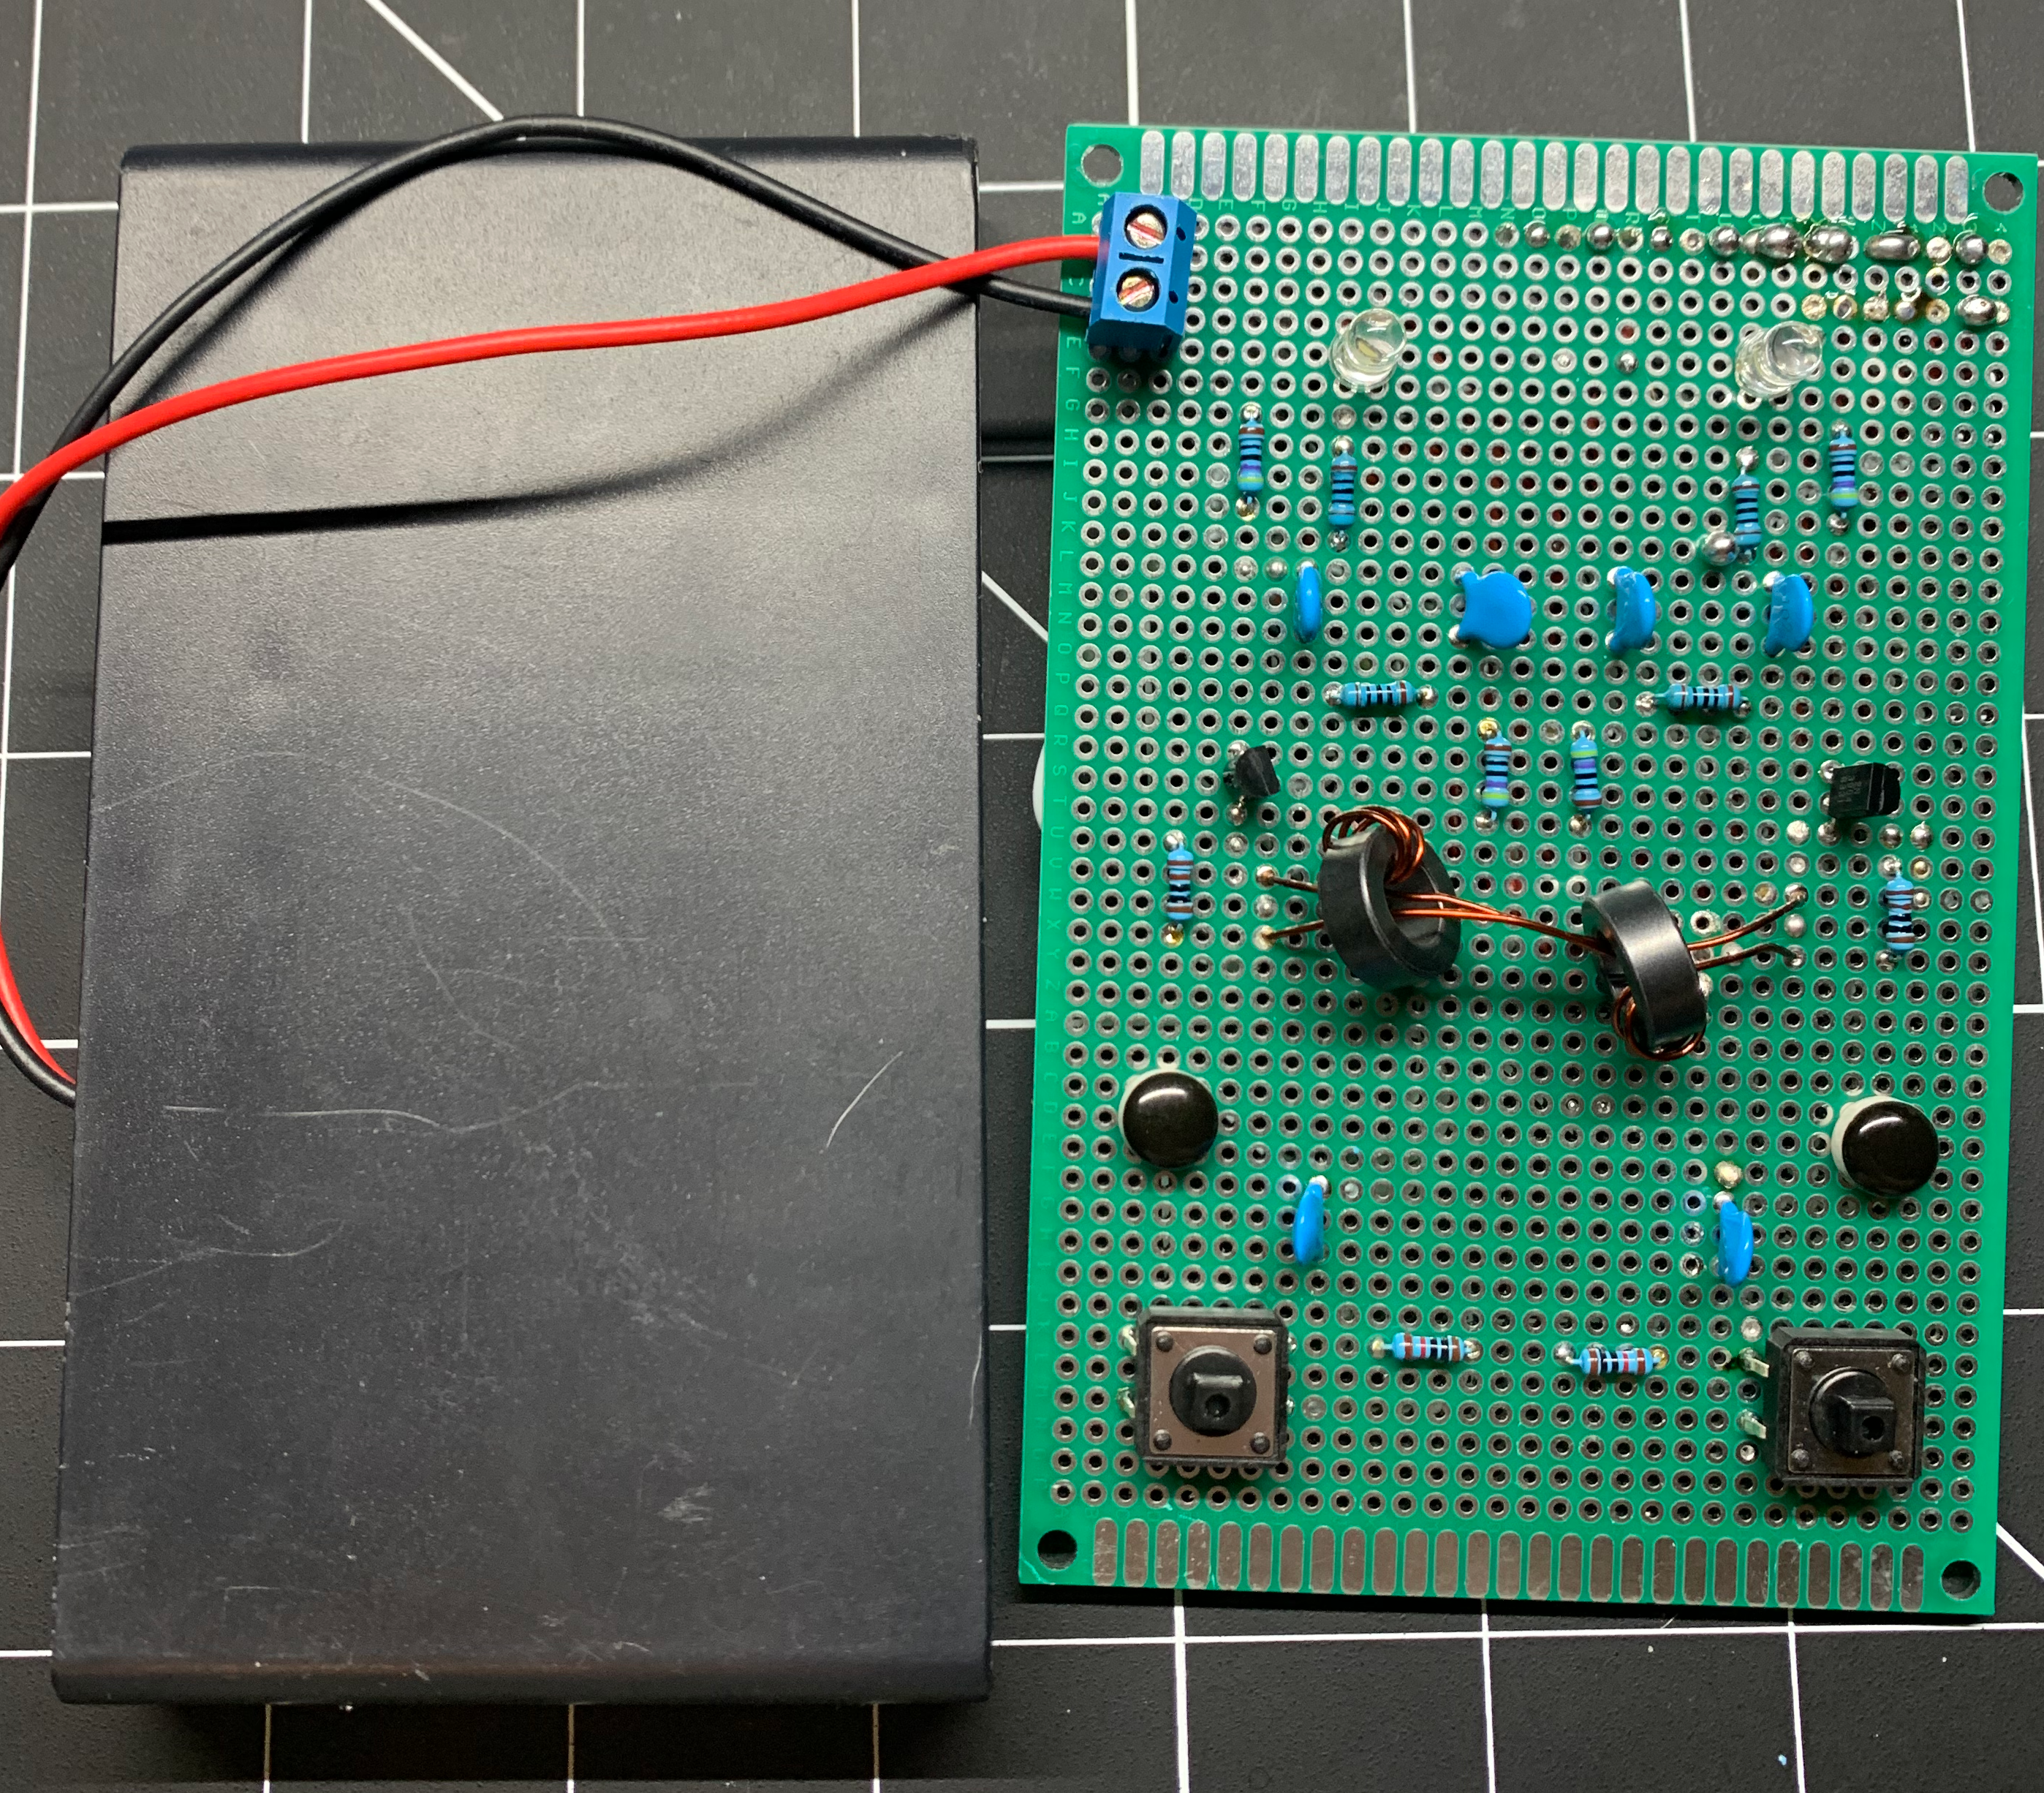
\includegraphics[width=5cm]{img/circuitfull.png}
  \caption{\small\emph{fig 7. The full circuit, off. The cores still keep their state even without power.}}
\end{figure}

\noindent Should this lab be conducted again, a more accurate form of measurement should be used. Specifically, the flux density of the field should be calculated relative to the distance and size of the ferrite core, and then compared to the theoretical values in sources 1, 3, and 4.

\newpage\section{References}
\begin{enumerate}
\item Papian, William. 1954. Review of The MIT Magnetic-Core Memory, MIT.
\item John David Jackson, and Wiley. 2011. Classical Electrodynamics. New Delhi: Wiley India.
\item C.J. Quartly. 1962. Square-Loop Ferrite Circuitry: Storage and Logic Techniques. Pearson-Hall.
\item Raymond Stewert-Williams. 1959. Magnetic Core Storage. Telemeter Magnetics.
\item Soshin Chikazumi. 2009. Physics of Ferromagnetism. Oxford Oxford Univ. Press.
\item Visintin-Trento, A. 2001. “Maxwell’s Equations with Vector Hysteresis.”
\item Farhat, Hassan A. 2004. Digital Design and Computer Organization. Boca Raton, Fl: Crc Press.
\item “Project Whirlwind | the MIT 150 Exhibition.” n.d. http://museum.mit.edu/150/21.
\item IEEE Journal of Solid State Circuits. 1969, p 288-291. Modified by Brek Martin.
\end{enumerate}

\end{document}